\documentclass[12pt, a4paper]{article}

\usepackage[T1, T2A]{fontenc}
\usepackage[utf8]{inputenc}
\usepackage[english, russian]{babel}
\usepackage{amsmath, amssymb}
\usepackage[left=3cm, right=1.5cm, top=2cm, bottom=2cm]{geometry}
\usepackage[displaymath]{lineno}
\usepackage[space]{cite}
\usepackage{xcolor, graphicx}

\usepackage{amsmath}
% Отключаем привязку нумерации к секциям в основном тексте
\counterwithout{equation}{section}
% Настройка для приложений
\usepackage{etoolbox}
\appto\appendix{%
	\renewcommand{\theequation}{П\arabic{equation}}%
	\setcounter{equation}{0}%
}


\renewcommand{\vec}{\mathbf}
\linenumbers
\linespread{2}

\def \eps {\varepsilon}
\def \w {\omega}
\def \ph {\varphi}
\def \kp { \varkappa}
\def \ex { \operatorname{ex}}
\def \out { \operatorname{out}}

\newcommand{\rd}[1]{\color{red} #1 \color{black}}

\newcommand{\op}[1]{\operatorname {#1}}

\newcommand{\dt}[1]{\frac{\partial {#1}}{\partial t}}
\newcommand{\dx}[1]{\frac{\partial {#1}}{\partial x}}
\newcommand{\dn}[1]{\left.\frac{\partial #1}{\partial \vec{n}}\right|_{ S}}
\newcommand{\dr}[1]{\left.\frac{\partial #1}{\partial r}\right|_{ r = a}}
\newcommand{\sumexp}[1]{\frac{{#1} e^{i \w t} + {#1}^* e^{-i \w t}}{2}}
\newcommand{\sumexptwo}[1]{\frac{{#1} e^{2 i \w t} + {#1}^* e^{-2 i \w t}}{2}}
\newcommand{\dtau}[1]{\frac{\partial {#1}}{\partial \tau}}
\begin{document}
\thispagestyle{empty}

 \ Контактные данные автора, ответственного за связь с редакцией\\
Павличенко Иван Александрович\\
Нижегородский госуниверситет им. Н.\,И. Лобачевского, 603022, г. Нижний Новгород, пр.Гагарина, 23\\
контактный телефон {+7 831 465-60-35}\\
e-mail: pavlichenko@rf.unn.ru 

\newpage
\setcounter{page}{1}

УДК 533.98{:}533.9...12
\begin{center}
\large\bf ВОЗБУЖДЕНИЕ ДВОЙНЫХ ПЛАЗМОННЫХ\\ РЕЗОНАНСОВ В СФЕРИЧЕСКОЙ МЕТАЛЛИЧЕСКОЙ\\НАНОЧАСТИЦЕ
\end{center}

И.\,А. Павличенко$^{1}$, М.\,Р. Удалов$^{1}$

$^1$ Нижегородский госуниверситет им. Н.\,И. Лобачевского, г. Нижний Новгород.\\

В работе теоретически исследуется нелинейное взаимодействие сферической металлической наночастицы с внешним электромагнитным полем с учетом пространственной дисперсии и возбуждения второй гармоники.
Впервые рассмотрен случай двойных плазмонных резонансов, когда одновременно частоты основной и удвоенной гармоник поля совпадают с частотой Ми и частотой одного из объемных плазмонов наночастицы, соответственно.
На основе гидродинамической модели рассчитана средняя мощность потерь энергии в объеме наночастицы.
Расчеты показали, что максимальное значение мощности потерь 
чувствительно к изменению величины диэлектрической проницаемости среды, окружающей наночастицу, и заметным образом возрастает при выполнении условий возбуждения двойных резонансов.
Полученные результаты показывают возможность использования данного эффекта для управления нелинейными оптическими свойствами наноструктур и нужд оптической диагностики.


\newpage
\begin{center}
{\large\bf EXCITATION OF DOUBLE PLASMON\\ RESONANCES IN A SPHERICAL METALLIC\\ NANOPARTICLE}
\end{center}

I.\,A. Pavlichenko, M.\,R. Udalov

In this paper, the interaction of electrons with phonons is investigated, with  patial dispersion and second harmonic generation taken into account.
For the first time, the case of double plasmon resonances is considered, where the frequencies of both the fundamental and doubled harmonic of the field simultaneously coincide with the Mie frequency and the frequency of one of the nanoparticle's volume plasmons, respectively.
Based on the hydrodynamic model, the average power loss in the nanoparticle volume was calculated.
The calculations show that the maximum power loss is sensitive to changes in the dielectric permittivity of the surrounding medium and increases significantly under double-resonance excitation conditions.
The obtained results demonstrate the potential use of this effect for controlling the nonlinear optical properties of nanostructures and for optical diagnostics.\\



\newpage

\section*{В\,В\,Е\,Д\,Е\,Н\,И\,Е}

Металлические наноструктуры привлекают к себе большое внимание благодаря своим уникальным характеристикам, связанным с возможностью возбуждения в них плазмонных резонансов на частоте падающего на наночастицу электромагнитного излучения.
Основной интерес к таким плазмонным наноструктурам обусловлен их способностью локализовать электромагнитные поля на нанометровых масштабах, существенно меньших дифракционного предела, что позволяет контролировать свойства оптического излучения на масштабах, намного меньших его длины волны \cite{Mai2007, Gram2010}.
Благодаря плазмонным резонансам в наноструктурах происходит существенное увеличение локальной плотности энергии поля, что приводит к возможности проявления в них различного рода нелинейных эффектов, таких как, например, многофотонная люминесценция \cite{Cas2011,biagioni2012,chen2021, ko2011}, четырехволновое смешивание \cite{danckwerts2007, harutyunyan2012,Li2016, paspalakis2014, singh2016} и генерация гармоник оптического излучения \cite{drobyh2020, smirnova2014, TorresTorres2010}.
В частности, явление генерации второй гармоники в наноструктурах  (возможность возникновения которого в ограниченных металлических объектах была впервые обнаружена экспериментально и объяснена теоретически в работах \cite{franken1961, Bloembergen1962}) является в настоящее время основой для широкого круга практических применений, включающего диагностику наноструктур и оптических сред (см., например, \cite{butet2015, Butet2012}).

Важным фактором, благодаря которому наноструктуры и основанные на них метаматериалы могут служить эффективным инструментом для генерации второй гармоники, является возможность резонансного усиления поля не только основной гармоники оптического излучения, но и его второй гармоники при совпадении удвоенной частоты с собственной частотой другой плазмонной модой наноструктуры. 
К настоящему моменту явление двойного плазмонного резонанса исследовалось фактически только для наноструктур, обеспечивающих одновременное возбуждение двух различных поверхностных плазмонов наночастицы на основной и удвоенной гармониках падающего излучения \cite{Ai2021,Thyagarajan2012}.
Однако в общем случае в наноструктуре помимо поверхностных плазмонов могут существовать и объемные плазмоны \cite{Elibol2022,Gildenburg2016,Ruppin1975,Gildenburg1965} -- моды коллективных электронных колебаний, представляющие собой стоячие плазменные (ленгмюровские) волны и возникающие из-за пространственной дисперсии. 
%(нелокальности поляризуемости плазмы).
 Объемные плазмоны, как известно, могут сильно проявлять себя в случае, когда источник возбуждения коллективных электронных колебаний находится внутри наночастицы и характеризуется неоднородным распределением поля, что, например, имеет место в задачах спектроскопии характеристических потерь энергии электронами (англ. Electron Energy Loss Spectroscopy) при прохождении  пучка заряженных частиц через объем наноструктуры
\cite{Gildenburg2016, Kryshtal2025}. 
Подобная ситуация может возникнуть и в задачах генерации второй гармоники, когда обусловленные нелинейностью токи второй гармоники, возбуждаемые при резонансе поверхностного плазмона на основной частоте колебаний, могут возбуждать объемные плазмонные колебания в наночастице. Данный эффект может иметь место, например, в случае наноструктуры простейшей формы, металлической сферической наночастицы, однако к настоящему моменту двойные плазмонные резонансы типа <<поверхностный плазмон -- объемный плазмон>> фактически не были исследованы и являются предметом исследования данной работы.

В данной работе на основании гидродинамического подхода \cite{Haas2011, Boardman1982, Manfredi2021} исследуются нелинейные эффекты, обусловленные возникновением резонансов объемных плазмонов на удвоенной частоте в условиях, когда частота основной гармоники наночастицы также испытывает резонанс и совпадает с частотой дипольного поверхностного плазмона наночастицы (резонанс Ми). Работа организована следующим образом: вначале на основе уравнений гидродинамики с использованием метода последовательных приближений сформулированы краевые задачи, описывающие в квазистатическом приближении пространственное распределение поля и плотности заряда на основной и удвоенной гармониках внешнего поля в малой металлической наночастице произвольной формы. Далее описано решение этих задач применительно к случаю сферической наночастицы, и исследованы условия отвечающие условию возбуждения в наночастицах двойных резонансов типа поверхностный плазмон – объемный плазмон. В последующем разделе приведены результаты расчетов, иллюстрирующие влияние исследуемых резонансов на частотные зависимости сечения поглощения сферических наночастиц и сформулированы основные результаты работы.


\section{ПОСТАНОВКА ЗАДАЧИ}

{Рассмотрим металлическую наночастицу }произвольной формы, находящуюся в заданном внешнем поле падающей электромагнитной волны, 
% на частоте $\w$ 
помещенную в среду с диэлектрической проницаемостью $\eps_d$. Как известно, достаточно подробное описание нелинейной динамики носителей в квазиклассическом приближении может быть получено с помощью набора уравнений гидродинамики (уравнение непрерывности и уравнение Эйлера), описывающих электронную плазму как сжимаемую заряженную жидкость  %https://doi.org/10.1002/lpor.201700082 
\cite{Boardman1982, Forstmann1986,Sipe1980,David2011}. 
При построении физической модели двойных резонансов исследуемого типа будем считать выполненными ряд приближений, а именно будем предполагать, что (I) 
выполнены условия применимости
квазистатического приближения для описания поля внутри и вблизи поверхности наночастицы и частица фактически находится во внешнем однородном переменном поле $\vec{E_0}e^{i\w t}$, (II) вклад в магнитную составляющую силы Лоренца, действующую на электроны в металле пренебрежимо мал, (III) электроны находятся внутри бесконечно глубокой потенциальной ямы, то есть будем пренебрегать эффектом размывания профиля электронной плотности близ границы металла (так называемый spill-out effect) \cite{Takeuchi2022,Jin2015,Zhou2021}, возникающим при учете давления электронов и (IV) положительный заряд ионного остова с равномерной плотностью распределен по объему наночастицы (предполагается, что в отсутствие внешнего поля электроны, как и ионы, распределены равномерно по объему частицы с плотностью $N_0$, а диэлектрическая проницаемость ионного остова материала частицы равна $\eps_\infty$). Описанные выше условия (вместе с условиями применимости гидродинамического подхода) приводят к следующим ограничениям на параметры задачи: 
\begin{equation} 	
\frac{v_F}{\omega_p} \ll L \ll \frac{2\pi c}{2\omega\sqrt{\eps_{d, \infty}}},  \quad v \ll c, 
\end{equation} 
где $v_F = \hbar (3 \pi^2 N_0)^\frac{1}{3}/m $ — скорость Ферми, $c$ — скорость света, $e$ и $m$ — заряд и масса электрона, $\hbar$ — постоянная Планка, $L$ — характерный размер частицы, $\w$ — частота внешнего поля, $ \w_p = 
\sqrt{4 \pi e^2 N_0 / m}$  — плазменная частота. Принимаемые здесь приближения несколько сужают область применимости рассматриваемой модели, однако поскольку ранее двойные плазмонные резонансы обсуждаемого здесь типа фактически не исследовались, такое упрощение модели представляется оправданным первым шагом на пути построения более точной модели. 

С учетом указанных предположений о характеристиках наночастицы и внешнего поля, нелинейная динамика коллективных электронных колебаний в наночастице подчиняется системе уравнений:
\begin{equation} 
	\label{непр}
	\dt{N} + \operatorname{div}(N \vec{v}) = 0,
\end{equation}
\begin{equation} 
	\label{гидр}
	\dt{\vec{v}} + \nu \vec{v} +(\vec{v} \nabla)\vec{v} = \frac{e}{m}\vec{E} - \frac{1}{mN} \nabla p, 
\end{equation}
\begin{equation} 
	\label{максв}
	\operatorname{div}\vec{E} = \frac{4\pi}{\eps_\infty}e(N-N_0),
\end{equation}
где введены следующие параметры электронов: $\vec{v}$ и $N$ – скорость и концентрация электронов в металле, $\nu$ – эффективная частота соударений, 
%$\vec{f} = N \vec{v}$ имеет смысл потока,
$p$ – давление электронов. Конкретный вид выражения для последней из перечисленных величин, фактически отвечающей за нелокальность поляризационного отклика плазмы, являлся предметом множества дискуссий и в настоящее время существует широкий спектр моделей, описывающих эту величину применительно к различным условиям. В рамках рассматриваемой здесь простой модели мы используем следующее феноменологическое уравнение состояния, отвечающее исследуемому здесь случаю быстрого адиабатического процесса и позволяющее получить из описанных выше уравнений (\ref{непр}), (\ref{гидр}) известный закон дисперсии как для поверхностных, так и для объемных плазмонов: 
\begin{equation}
	\label{p}
 p = p_0 (N/N_0)^\gamma, \quad p_0 = m v_F^2 N_0/5, \quad \gamma = 3.
\end{equation}
Следуя обычной процедуре метода возмущений, применяемого в случае слабой нелинейности, представим в уравнениях неизвестные плотность электронов, скорость и напряженность поля в виде суммы гармонических слагаемых, изменяющихся на частотах, кратных частоте внешнего поля. Далее сопоставляя в получившихся уравнениях величины одинакового порядка малости, получаем следующие уравнения
\begin{equation} 
	\label{rho_sys}
 \Delta \rho_{n} + k_{pn}^2\rho_{n} = -\frac{1}{4 \pi r_0^2} \Delta \ph^{(\ex)}_{n} + \left( k_{pn}^2 + \frac{1}{r_0^2\eps_\infty}\right) {\rho^{(\ex)}_{n},}
\end{equation}
\begin{equation} 
	\label{phi_sys}
 \Delta \ph_{n} = - \frac{4 \pi}{\eps_\infty} \rho_{n}, \quad n = 1,2,
\end{equation}
определяющие комплексные амплитуды плотности заряда и потенциала поля для основной ($n=1$, $\w_1=\w$) и удвоенной ($n=2$, $\w_2=2\w$) гармоник.
В выражениях выше величина $r_0 = \sqrt{3}v_F/(\sqrt{5}\w_p)$ имеет смысл характерного радиуса нелокальности плазмы (с точностью до коэффициента совпадает с длиной Томаса-Ферми) и  
\begin{equation} 
k_{pn} = \sqrt{\frac{5[\w_{n}(\w_{n} - i\nu) - \w_p^2/\eps_\infty]}{3v_F^2}} 
\end{equation}
-- волновое число продольной волны.
Введенные в уравнениях (\ref{rho_sys}), (\ref{phi_sys}) величины $\ph^{(\ex)}_{n}$ и $\rho^{(\ex)}_{n}$ играют фактически роль расположенных внутри плазмы сторонних источников колебаний. Для первой гармоники они, очевидно, тождественно равны нулю ($\ph^{(\ex)}_1\equiv0$, $\rho^{(\ex)}_1\equiv0$) и введены только для более краткой и единой записи результирующих уравнений. Для колебаний второй гармоники сторонние источники $\ph^{(\ex)}_2$, $\rho^{(\ex)}_2$ определяются следующим выражением 
\begin{equation}
	\label{rho_ex}
 - 2i\w \rho^{(\ex)}_2 = \frac{1}{2}\operatorname{div} \rho_1 \vec{v_1},
\end{equation}
\begin{equation}
	\label{phi_ex}
\ph^{(\ex)}_2 = \frac{m}{4e}\left(\frac{v_0^2}{N_0^2}N_1^2 + \vec{v}_1^2\right),
\end{equation}
и фактически имеют смысл сторонней плотности заряда (возникающей из-за нелинейного слагаемого в уравнении непрерывности (\ref{непр})) и потенциала стороннего поля, (возникающего из-за нелинейности уравнения состояния (\ref{p}) и из-за конвективного члена в уравнении (\ref{гидр})), осциллирующих на удвоенной частоте. 

Система уравнений (\ref{phi_sys}), (\ref{rho_sys}) должна быть дополнена граничными условиями на поверхности наночастицы. Первые из используемых нами граничных условий, вытекают непосредственно из уравнений Максвелла
\begin{equation} 
	\label{g_u1}
	\left. \ph_n \right|_{ S} = \left. \ph_n^{(\out)} \right|_{ S} 
\end{equation}
\begin{equation} 
	\label{g_u2}
	\eps_\infty \dn{\ph_n} = \eps_d \dn{\ph_n^{(\out)}},
\end{equation}
($S$ -- поверхность наночастицы, $\vec{n}$ -- вектор нормали к этой поверхности) и связывают потенциалы электрического поля внутри наночастицы с соответствующими потенциалами $\ph_{n}^{(\out)}$ в окружающем ее однородном диэлектрике.
Последнее, необходимое для однозначного решения сформулированных уравнений, граничное условие определяется характером движения электронов близ границы наночастицы. В случае принимаемого здесь условия зеркального отражения электронов от поверхности металла соответствующее граничное условие приобретает вид

\begin{equation} 
	\label{psi}
\dn{\psi_n}	= 0, \quad \psi_n = \ph_n + 4 \pi r_0^2 \rho_n + \ph^{(\ex)}_n, 
\end{equation}
где $\psi_{n}$ по сути имеют смысл потенциала скорости электронов на основной и удвоенной гармониках колебаний:
\begin{equation} 
	\label{v}
	\vec{v}_n = -\frac{e}{i(\w_n - i\nu)m} \nabla \psi_n.
\end{equation}

Сформулированная система уравнений, как и в других работах, посвященных исследованию генерации второй гармоники в условиях двойных резонансов (см., например, \cite{Ai2021, HuaGersten1986, Panoiu2018, Beer2022}), позволяет рассчитать структуру колебаний. Основным новым элементом здесь является здесь учет нелокальности поляризации плазмы не только для основной, но и для удвоенной гармоники, что позволяет описать возникновение резонансов объемных плазмонов на ее частоте. Как известно, поле объемных плазмонов сильно локализовано внутри наночастицы и соответствующие им резонансы обычно слабо проявляется в спектрах рассеянного излучения, однако как будет показано далее, возбуждение объемных плазмонов на удвоенной частоте может приводить к заметному изменению поглощаемой наночастицей мощности. Расчет спектров поглощения в рамках рассматриваемой модели может быть выполнен следующим образом. Потери энергии обусловлены наличием в уравнении (\ref{гидр}) диссипативной силы, с плотностью $m \nu N \vec{v}$. Средняя за период плотность мощности этой силы очевидным образом может быть выражена через комплексные амплитуды плотностей потока и скоростей первой и второй гармоник. Интегрируя по объему наночастицы с учетом соотношений (\ref{rho_sys}), (\ref{phi_sys}) и граничного условия (\ref{psi}), приходим к следующему выражению для средней за период мощности потерь во всем объеме наночастицы: 
\begin{equation} 
	\label{Q}
	Q = \frac{\nu}{2}\mathrm{Re}  \sum_{n=1,2}\frac{\w_n}{i(\w_n - i \nu)}\iiint\rho_n \psi_n^* dV.
\end{equation}

\section{ДВОЙНЫЕ РЕЗОНАНСЫ В СФЕРИЧЕСКОЙ НАНОЧАСТИЦЕ}
Применительно к сферической наночастице радиуса $a$, помещенной в однородную среду с проницаемостью $\eps_d$, решение линейной задачи, описывающей колебания на частоте внешнего поля, хорошо известно (см., например, \cite{HuaGersten1986}) и выражается через сферические функции Бесселя $j_n$. Как можно показать, выражения для потенциала и плотности заряда в этом случае имеют следующий вид
\begin{equation} 
	\label{C}
	C= \frac{-3\eps_d E_0}{\eps + 2\eps_d [1 + (\eps/\eps_\infty - 1) G_1(a) ]},  
\end{equation}
%\begin{equation} 
%\rho_{01} = \frac{\eps -1}{4\pi}k_{p1}\frac{C}{j_1' (k_{p1}a)}, 	
%\end{equation}
\begin{equation} 
	\label{rho_and_phi}
	\rho_1 = C \frac{-k_{p1}^2a\w_p^2}{4\pi\w(\w - i \nu) } G_1(r)\cos\theta, \quad \ph_1 = C r + \frac{4\pi \rho_1 }{(k_{p1}a)^2 \eps_\infty},
\end{equation}
\begin{equation}
	\label{eps_and_G}
		 G_m(r) =\frac{j_m(k_{p1}r)}{k_{p1}a j_m'(k_{p1}a)},\quad
	\eps = \eps_\infty - \frac{\w_p^2}{\w(\w - i\nu)},
\end{equation}
где $a$ -- радиус наночастицы, $\theta$ и $r$  -- полярный угол (отсчитываемый от направления внешнего поля) и расстояние от центра наночастицы, соответственно. Последняя из величин (\ref{eps_and_G}) имеет смысл диэлектрической проницаемости металла в отсутствие нелокальности. Как можно увидеть из выражения (\ref{C}),  в рассматриваемой
системе возможны резонансы, обусловленные совпадением частоты
внешнего напряжения с частотами собственных плазмонных колебаний.
Положение резонансных максимумов определяется близостью к нулю знаменателя в уравнении (\ref{C}). 
%В общем случае присутствует один резонанс на частоте лежащей ниже плазменной (поверхностный плазмон) и серия резонансов на частотах, превышающих плазменную частоту (объемные плазмоны).
Наиболее сильный из них, дипольный поверхностный плазмон (резонанс Ми), без учета пространственной дисперсии, зависит от диэлектрической проницаемости внешней среды, определяется выражением $\w^{(1,0)} \approx \w_p / \sqrt{\eps_\infty + 2\eps_d}  $, и частота генерируемой в наночастице второй гармоники колебаний может лежать в области частот, отвечающей возможности возбуждения объемных плазмонов. Значения их резонансных частот определяются общим дисперсионным уравнением:
\begin{equation}
	\label{freq_eq} 	
m \eps + \eps_d(m+1)(1 + m (\eps/\eps_\infty - 1) G_m) = 0,	
\end{equation}
($m=0,1,2,...$ – номер мультиполя), которое может быть также получено из решения однородной краевой задачи (\ref{rho_sys})-(\ref{psi}) в отсутствие внешнего поля. В интересующем нас случае слабой пространственной дисперсии $r_0 \ll a$ значения резонансных частот слабо зависят от параметров окружающей среды и приближенно могут быть найдены из соотношения 
\begin{equation} 
 \w^{(m,k)}(\w^{(m,k)} - i \nu) \approx \left(\frac{\eta^{(m,k)} v_F }{a}\right)^2 \frac{3}{5} + \frac{\w_p^2}{\eps_\infty},
\end{equation}
где $\eta^{(m,k)}$ -- $k$-й корень сферической функции Бесселя порядка $m+1$.	Из всех возможных условий двойных резонансов здесь представляет интерес рассмотрение случая с $m=0$ и $m=2$ (монопольные и квадрупольные объемные резонансы соответственно), поскольку в случае сферической наночастицы, как можно увидеть из вида выражений для сторонних источников поля второй гармоники (\ref{rho_ex}) (\ref{phi_ex}), они  могут возбуждать только колебания монопольного и квадрупольного типов.
Возможность возбуждения двойных резонансов при изменении диэлектрической проницаемости внешней среды проиллюстрированы на рисунке \ref{fig_w}, где изображены зависимости резонансной частоты дипольного поверхностного плазмона $\w^{(1,0)}$ от величины $\eps_d$, при типичных для металлических наночастиц значениях параметров $v_F = 1.5 \cdot 10^8$ см/c, $\w_p = 5$ эВ, $\nu / \w_p = 0.02$. 
На графике также отмечены корни уравнения $2\w^{(1,0)}=\w^{(m,k)}$, отвечающие условиям возбуждения двойных резонансов.
При уменьшении проницаемости $\eps_d$ частота второй гармоники $\w_2=2\w^{(1,0)}$ поочередно совпадает с частотами различных объемных монопольных и квадрупольных мод, что, как мы увидим далее, приводит к заметному возрастанию мощности потерь. 
%Расстояние между положениями резонансов определяется отношением $r_0/a$: чем больше $r_0/a$, тем больше расстояние между резонансами. При этом, чтобы были различимы отдельные резонансы, они должны отличаться по частоте больше чем на характерную ширину линии потерь. Таким образом, условием сильной выраженности резонансов будет являться следующее выражение: $\nu/\w_p \ll r_0/a$.

На основании дисперсионного соотношения (\ref{freq_eq}) также могут быть определены мнимые части резонансных частот (декременты затухания) всех плазмонных мод наночастицы, которые в рамках рассматриваемой простой модели все оказываются равными $\nu/2$.
В то же время, известно в случае сферических наночастиц, что основные механизмы потерь (внутренние, поверхностные и радиационные потери) вносят различный вклад в декременты затухания различных мультипольных поверхностных и объемных резонансов. Ввиду предположения о малости размера частицы по сравнению с длиной волны внешнего излучения мы здесь можем пренебречь радиационными потерями, однако (в интересующем нас случае наночастицы малых размеров) поверхностные потери могут приводить к заметному увеличению декремента затухания резонанса дипольного поверхностного плазмона. Учет этих потерь проводится здесь известных образом: при решении задачи о колебаниях на основной частоте $\w_1$ эффективная частота столкновений $\nu$ заменялась величиной равной $\nu_{\op{dip}} = \nu + 3 v_F / (4a \w_p)$ \cite{Hovel1993}. При решении части задачи, описывающей колебания на удвоенной частоте $\w_2$, учет дополнительных механизмов потерь фактически не требуется, поскольку для всех мультипольных объемных плазмонов вклады в ширины их резонансных линий, вносимые поверхностными и радиационными потерями оказываются оказываются $\sim(r_0/a)^5$ и пренебрежимо малы \cite{Gildenburg2016}.


При решении задачи о колебаниях на удвоенной частоте можно заметить, что различные слагаемые в выражениях для сторонних источников
\begin{equation} 	
	\ph^{(\ex)}_2 = \frac{e}{4 \pi \w_p^2}\left[(4\pi)
	^2r_0^2\rho_1^2 - \frac{\w_p^2}{(\w - i \nu)^2}(\nabla \psi_1)^2\right], 
\end{equation}

\begin{equation} 	
	\rho^{(\ex)}_2 = \frac{e}{4 m \w(\w - i \nu)}\left(-4 \pi \rho_1^2 \frac{w(\w - i \nu)}{\w_p^2} + \nabla \psi_1\nabla \rho_1\right),
\end{equation}
определяемые произведениями плотности заряда $\rho_1$  и потенциала $\psi_1$ при дипольных ($\sim\cos\theta$) колебаниях и их пространственных производных, содержат зависимость от угловой координаты либо $\cos^2\theta$, либо  $\sin^2\theta$. Последнее позволяет представить эти величины в виде произведений радиальных функций $F_{m}^{\ph,\rho}(r)$ на полиномы Лежандра $P_m$:
\begin{equation}
	\label{P_phi_ex} 	
	\ph^{(\ex)}_2 =\sum_{m=0,2} F_m^\ph(r)P_m(\cos\theta),
\end{equation}
\begin{equation} 
	\label{P_rho_ex} 	
	\rho^{(\ex)}_2 =\sum_{m=0,2} F_m^\rho(r)P_m(\cos\theta).
\end{equation}
В силу ортогональности полиномов Лежандра и линейности уравнений (\ref{rho_sys}),(\ref{phi_sys}), неизвестные плотность заряда и потенциал второй гармоники могут быть также представлены в виде монопольной и квадрупольной составляющих 
\begin{equation} 	
	\ph_2 =\sum_{m=0,2} R_m(r)P_m(\cos\theta),
\end{equation}
\begin{equation} 	
	\rho_2 =\sum_{m=0,2} \Phi_m(r)P_m(\cos\theta),
\end{equation}
где $R_{m}$, $\Phi_{m}$ -- неизвестные радиальные функции. При этом система уравнений в частных производных  (\ref{rho_sys}),(\ref{phi_sys}) распадается на две независимые системы обыкновенных дифференциальных уравнений, описывающих эти две мультипольные составляющие колебаний
\begin{equation}
	\label{P_sys1}  	
	(\hat L_m + \kp_p^2) R_m = -\frac{1}{4 \pi r_0^2}\hat L_m F_m^\ph  + \frac{2\w(2\w - i \nu)}{\w_p^2r_0^2}F_m^\rho,
\end{equation}
\begin{equation} 
	\label{P_sys2} 	
	\hat L_m \Phi_m = -\frac{4\pi}{\eps_\infty}R_m,  \quad \hat{L}_m = \frac{1}{r^2} \frac{\partial}{\partial r} \left( r^2 \frac{\partial}{\partial r} \right) - \frac{m(m+1)}{r^2}.
\end{equation}
по-отдельности. Далее, пользуясь тем, что общий вид выражения для потенциала квадрупольных и монопольных колебаний вне сферической частицы известен, получаем из (\ref{g_u1})-(\ref{g_u2})  граничные условия для радиальных функций 
\begin{equation}
\Phi_0(r=a) = 0,~~	\left.\left( \Phi_2 + \frac{r\varepsilon_\infty}{3\varepsilon_d} \frac{\partial}{\partial r} \Phi_2 \right) \right|_{r=a} = 0.
	\label{eq:potential_condition}
\end{equation}
\begin{equation}
	\label{g_u_rad_Vn}
	\left.\frac{\partial}{\partial r} \left( \Phi_m + 4\pi r_0^2 R_m + F_m^{\varphi} \right) \right|_{r=a} = 0.
\end{equation}
Краевая задача (\ref{P_sys1})--(\ref{g_u_rad_Vn}) решалась численно на основе методов Галеркина и матричной прогонки. Получив значения радиальных функций, мощности потерь, отвечающие мнонопольным и квадрупольным колебаниям, рассчитывались на основании выражений 
\begin{equation} 	
	Q_{m} = \frac{2\pi\nu}{2m+1}\mathrm{Re} \frac{2\w}{i(2\w - i \nu)} \int\limits_0^a R_m(\Phi_m  + 4\pi r_0^2R_m + F_m^\ph)^*r^2dr, \quad m=0,2,
\end{equation}
вытекающих из соотношения (\ref{Q}). Полная средняя за период колебаний мощность потерь $Q$, очевидно, представима в виде $Q = \sum_{m=0}^2 Q_m$, где вклад дипольной составляющей
\begin{equation} 
	Q_1 = \frac{2\pi\nu}{3} \mathrm{Re} \frac{\w}{i(\w - i\nu)} \int\limits_{0}^{a} R_{1}(\Phi_{1} + 4\pi r_{0}^{2}R_{1})^{*}r^{2}dr.
\end{equation}
\section{РЕЗУЛЬТАТЫ РАСЧЕТОВ}

На рисунках \ref{fig1_epsd2}, \ref{fig1_epsd4} проиллюстрированы зависимости мощности потерь от частоты при различных значениях проницаемостей $\eps_\infty$ и $\eps_d$ и тех же модельных значениях параметров наночастицы, что и на рисунке 1. Как видим, при двойных резонансах мощности потерь, обусловленные монопольными и квадрупольными колебаниями на удвоенной частоте (пунктирные и штрих-пунктирные кривые, соответственно) вносят заметный вклад в полную мощность (сплошные кривые), приводя к изменению формы резонансной линии и максимального значения мощности по сравнению с линейным случаем (точечные кривые). Наиболее сильно этот эффект проявляется в случае возбуждения низших объемных мод (при больших значениях проницаемости $\eps_d$) и, что особенно интересно отметить, имеет место при резонансе только монопольных колебаний, обычно не проявляющих себя в задачах взаимодействия лазерного излучения с наночастицами. С уменьшением проницаемости окружающей среды $\eps_d$ и, соответственно, увеличением индексов возбуждаемых объемных мод, вклад в полную мощность потерь от резонансов второй гармоники убывает ввиду уменьшения их коэффициентов возбуждения. Последнее обусловлено тем, что токи, возбуждающие вторую гармонику колебаний наиболее сильны вблизи границы наночастицы (так же, как и поле дипольного поверхностного плазмона), а поле объемных плазмонных колебаний (фактически представляющих собой стоячие сферические продольные волны) с увеличением номера резонанса все сильнее сосредоточено в центре наночастицы.

Говоря о возможности возбуждения исследуемого типа двойных резонансов в реальных наночастицах, по-видимому следует отметить, что их возникновение невозможно в случае наиболее <<традиционных>> для наноплазмоники металлов (серебро и золото), поскольку они характеризуются существенным увеличением внутренних потерь в области возбуждения объемных плазмонов ($\textrm{Re}\eps \approx 0$), что ведет к фактически полному их подавлению при возбуждении оптическим полем.
В то же время, двойные резонансы по-видимому могут проявлять себя в случае наночастиц из натрия, -- металла, обладающего рядом преимуществ для применения в наноплазмонике по сравнению с благородными металлами (см, например \cite{Arboleda2016, Blaber2009}).
В качестве иллюстрации, на рисунке \ref{natr} изображены зависимости максимальной мощности потерь $Q_\textrm{max} = \max\{Q(\w)\}$ от проницаемости $\eps_d$ для натриевых наносфер (при $v_F = 1.07\cdot10^8$ см/с, $\w_p = 5.71$ эВ, $\nu = 0.03$ эВ \cite{ Blaber2009}) радиуса 10 нм и 7 нм при интенсивности внешнего поля $10^8$ $\text{Вт}/\text{см}^2$ и при интенсивности $5 \cdot 10^7$ $\text{Вт}/\text{см}^2$ для наночастицы радиуса 5 нм.
Как видим, при параметрах, представляющихся вполне реалистическими для задач наноплазмоники, двойные резонансы могут проявлять себя и могли бы послужить основой для практических приложений. 

Также важно отметить, что описываемые резонансы, наиболее сильно выраженные в представленных расчетах при значениях $\eps_d \sim 1\div2$ (нетипичных для известных оптических сред), могут проявляться и в случае сферических металлических наночастиц, покрытых слоем диэлектрика.
Как может быть показано на основании уравнений (\ref{rho_sys}), (\ref{phi_sys}) в случае металло-диэлектрической наноструктуры типа ядро-оболочка, дисперсионное соотношение (\ref{freq_eq}) оказывается справедливым, если заменить в нем диэлектрическую проницаемость внешней среды $\eps_d$ эффективным значением, 
\begin{equation} 	
%\textrm{ПРАВИЛЬНАЯ ФОРМУЛА,}
\eps_d^{(\operatorname{eff})} = \eps_s \frac{1-K_m}{1 + (m+1)K_m/m}, \quad K_m = (\frac{a}{b})^{2m+1} \frac{\eps_d - 1}{\eps_d + (m+1)/m},
\end{equation}
определяемым параметрами оболочки (ее диэлектрической проницаемости $\eps_s$ и внутренним и внешним радиусами $a$ и $b$). Таким образом исследуемые двойные резонансы в принципе могут использоваться для контроля размеров оболочки при создании такого типа наночастиц.


\section{ЗАКЛЮЧЕНИЕ}

В работе продемонстрировано, что в сферических металлических наноструктурах возможно возникновение нелинейных резонансных явлений, связанных с одновременным возбуждением дипольного поверхностного плазмона на частоте внешнего поля и объемных плазмонов на второй гармонике, возбуждаемой при его нелинейном взаимодействии с наночастицей. Проведенные расчеты демонстрируют, что одновременное резонансное усиление и основной и удвоенной гармоник поля приводит к увеличению мощности, поглощаемой наночастицей, приводя к изменению  формы резонансных линий и положения максимума ее на частотных зависимостях. Показано, что исследуемые двойные резонансы чувствительны к параметрам среды, окружающей наночастицу, и могут служить основой для нужд диагностики наночастиц и оптических сред.

\section{БЛАГОДАРНОСТИ}
Работа выполнена при поддержке Министерства науки и высшего образования Российской Федерации (государственное задание FSWR–2023–0031).
\newpage






\newpage
\begin{thebibliography}{99}
%\bibitem{} \cite{}
%A
\bibitem{Mai2007}
Maier S.~A. Plasmonics: Fundamentals and Applications. New York: Springer, 2007. 229~p.
\bibitem{Gram2010}
Gramotnev D.~K., Bozhevolnyi S.~I. // Nat. Photonics. 2010. V.~4. P.~83--91. doi: 10.1038/nphoton.2009.282

%multiphoton excited luminescence 
\bibitem{Cas2011}
Castro-Lopez M., Brinks D., Sapienza R., van Hulst N.~F. // Nano Lett. 2011. V.~11. P.~4674--4678. doi: 10.1021/nl202255g
\bibitem{biagioni2012}
Biagioni P., Brida D., Huang J.-S., et al. // Nano Lett. 2012. V. 12, No. 7. P. 2941–2946. doi: 10.1021/nl300616s.
\bibitem{chen2021}
Chen H., Sun M., Ma J., et al. // ACS Photonics. 2021. V. 8, No. 4. P. 1084–1092. doi: 10.1021/acsphotonics.0c01747.
\bibitem{ko2011}
Ko K.D., Kumar A., Fung K.H., et al. // Nano Lett. 2011. V. 11, No. 1. P. 61–65. doi: 10.1021/nl102751m.

%four-wave mixing 
\bibitem{danckwerts2007}
Danckwerts M., Novotny L. // Phys. Rev. Lett. 2007. V. 98. 026104. doi: 10.1103/PhysRevLett.98.026104.
\bibitem{harutyunyan2012}
Harutyunyan H., Volpe G., Quidant R., et al. // Phys. Rev. Lett. 2012. V. 108. 217403. doi: 10.1103/PhysRevLett.108.217403.
\bibitem{Li2016}
Li J.-B., Liang S., Xiao S., He M.-D., Kim N.-C., Chen L.-Q., Wu G.-H., Peng Y.-X., Luo X.-Y., Guo Z.-P. // Opt. Express. 2016. V.~24. P.~2360--2369. doi: 10.1364/OE.24.002360
\bibitem{paspalakis2014}
E. Paspalakis, S. Evangelou, S. G. Kosionis, and A. F. Terzis, {J. Appl. Phys.}, vol. 115, no. 8, p. 083106, 2014, doi: 10.1063/1.4866424.
\bibitem{singh2016}
S. K. Singh, M. Kurtulus Abak, and M. E. Tasgin, {Phys. Rev. B}, vol. 93, no. 3, p. 035410, 2016, doi: 10.1103/PhysRevB.93.035410.

%ВТ гарм 
\bibitem{drobyh2020}
E. Drobnyh and M. Sukharev, {J. Chem. Phys.}, vol. 152, no. 9, p. 094706, 2020, doi: 10.1063/1.5143238.
\bibitem{smirnova2014}
D. A. Smirnova, I. V. Shadrivov, A. E. Miroshnichenko, A. I. Smirnov, and Y. S. Kivshar, {Phys. Rev. B}, vol. 90, no. 3, p. 035412, 2014, doi: 10.1103/PhysRevB.90.035412.

%ТР гарм
\bibitem{TorresTorres2010}
Torres-Torres~C. // Int. J. Nanomedicine. 2010. P.~925. doi: 10.2147/ijn.s12463

%[5, 6]
\bibitem{franken1961}
P. A. Franken, A. E. Hill, C. P. Peters, and G. Weinreich, {Phys. Rev. Lett.}, vol. 7, no. 7, pp. 118–119, 1961, doi: 10.1103/PhysRevLett.7.118.
\bibitem{Bloembergen1962} 
Bloembergen~N., Pershan~P.~S. // Phys.~Rev. 1962. V.~128, No.~2. P.~606--622. 
doi: 10.1103/physrev.128.606

%[см эксп обзор] 
\bibitem{butet2015}
J. Butet, P.-F. Brevet, and O. J. F. Martin, {ACS Nano}, vol. 9, no. 11, pp. 10545–10562, 2015, doi: 10.1021/acsnano.5b04373.

%[7]
\bibitem{Butet2012}
Butet~J., Russier-Antoine~I., Jonin~C. и~др. // Nano Lett. 2012. V.~12, No.~3. P.~1697--1701. doi: 10.1021/nl300203u

\bibitem{Ai2021}
Ai~Q., Sterl~F., Zhang~H., Wang~J., Giessen~H. // ACS Nano. 2021. V.~15, No.~12. P.~19409--19417. doi: 10.1021/acsnano.1c05970
\bibitem{Thyagarajan2012}
Thyagarajan~K., Rivier~S., Lovera~A., Martin~O.~J.~F. // Opt. Express. 2012. V.~20, No.~12. P.~12860--12870. doi: 10.1364/OE.20.012860

%объемные плазмоны [] 
\bibitem{Gildenburg1965}
Gildenburg~V.~B., Kondrat’ev~I.~G. // Radio Eng. Electr. Phys. 1965. V.~10, No.~4. P.~560.
\bibitem{Ruppin1975}
Ruppin~R. // Phys. Rev. B. 1975. V.~11, No.~8. P.~2871--2876. doi: 10.1103/physrevb.11.2871.
\bibitem{Gildenburg2016}
Gildenburg~V.~B., Kostin~V.~A., Pavlichenko~I.~A. // Phys. Plasmas. 2016. V.~23, No.~3. Art. no.~032120. doi: 10.1063/1.4944395.





\bibitem{Elibol2022}
Elibol~K., Downing~C., Hobbs~R.~G. // Nanotechnology. 2022. V.~33, No.~47. Art. no.~475203. doi: 10.1088/1361-6528/ac8812.
\bibitem{Kryshtal2025}
Kryshtal~A., Khshanovska~O. // Sci. Rep. 2025. V.~15. Art. no.~5335. doi: 10.1038/s41598-025-88496-1.

%гидродинамической модели [] 
\bibitem{Haas2011}
Haas~F. Quantum plasmas: An hydrodynamic approach. New York : Springer, 2011. 65~p.
\bibitem{Boardman1982}
Electromagnetic surface modes / ed. by A.~D.~Boardman. Chichester : Wiley, 1982. 770~p.
% политропа
\bibitem{Manfredi2021}
Manfredi~G., Hervieux~P.-A., Hurst~J. // Rev. Mod. Plasma Phys. 2021. V.~5. P.~7. 
doi: 10.1007/s41614-021-00056-y


%ОБЗ_ТЕОР_ГД _12–15
\bibitem{Forstmann1986}
Forstmann~F., Gerhardts~R.~R. Metal Optics Near the Plasma Frequency. Berlin : Springer-Verlag, 1986. 132~p.
\bibitem{Sipe1980}
Sipe~J.~E., So~V.~C.~Y., Fukui~M., Stegeman~G.~I. // Phys. Rev. B. 1980. V.~21. P.~4389--4396. doi: 10.1103/PhysRevB.21.4389
\bibitem{David2011}
David~C., Garc\'{i}a de Abajo~F.~J. // J. Phys. Chem. C. 2011. V.~115. P.~19470--19477. doi: 10.1021/nn5038527
%spill-out effect
\bibitem{Takeuchi2022}
Takeuchi~T., Yabana~K. // Phys. Rev. A. 2022. V.~106. Art. no.~063517. doi: 10.1103/PhysRevA.106.063517
\bibitem{Jin2015}
Jin~D., Hu~Q., Neuhauser~D., von Cube~F., Yang~Y., Sachan~R. [et al.] // Phys. Rev. Lett. 2015. V.~115, No.~19. Art. no.~193901. doi: 10.1103/PhysRevLett.115.193901
\bibitem{Zhou2021}
Zhou~Q., Li~W., Zhang~P., Chen~X.-W. Calibrating quantum hydrodynamic model for noble metals in nanoplasmonics [physics.optics]. arXiv:2112.10099. 2021. doi: 10.48550/arXiv.2112.10099

\bibitem{HuaGersten1986}
Hua X. M., Gersten J. I. // Phys. Rev. B. 1986. V. 33, No. 6. P. 3756.


\bibitem{Panoiu2018}
Panoiu~N.~C., Sha~W.~E.~I., Lei~D.~Y., Li~G.-C. // J. Opt. 2018. V.~20, No.~8. Art. no.~083001. doi: 10.1088/2040-8986/aac8ed
\bibitem{Beer2022}
Beer~S., Gour~J., Alberucci~A., David~C., Nolte~S., Zeitner~U.~D. // Opt. Express. 2022. V.~30, No.~22. P.~40884--40894. doi: 10.1364/OE.470578

\bibitem{Hovel1993}
H\"{o}vel~H., Fritz~S., Hilger~A., Kreibig~U., Vollmer~M. // Phys. Rev. B. 1993. V.~48, No.~24. P.~18178--18188. doi: 10.1103/PhysRevB.48.18178
%# Sodium cluster and field params #
\bibitem{Arboleda2016}
Arboleda~D.~M., Santillán~J.~M.~J., Mendoza Herrera~L.~J., Muraca~D., Schinca~D.~C., Scaffardi~L.~B. // J. Phys. D: Appl. Phys. 2016. V.~49, No.~7. Art. no.~075302. doi: 10.1088/0022-3727/49/7/075302
\bibitem{Blaber2009}
Blaber~M.~G., Arnold~M.~D., Ford~M.~J. // J. Phys. Chem. C. 2009. V.~113, No.~8. P.~3041--3045. doi: 10.1021/jp810808h
%fig1_epsd4.eps
\end{thebibliography}

\newpage
\section{РИСУНКИ И ТАБЛИЦЫ}
\begin{figure}[h]
	\centering
	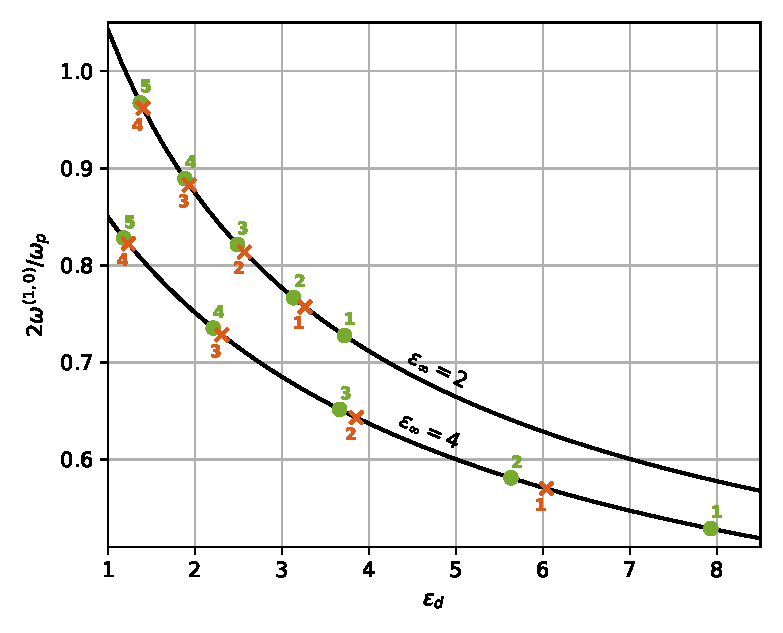
\includegraphics[width=80mm]{./image/fig_w.eps}
	\caption{Положение частоты основного дипольного поверхностного резонанса (сплошная линия) в зависимости от диэлектрической проницаемости внешней среды, а также положения резонансных частот при $m=0,2$, для монопольных (точечный маркер) и квадрупольных (крестообразный маркер) объемных резонансов соответственно, при разной диэлектрической проницаемости ионного остова. Числом при маркере обозначен порядковый номер соответствующего резонанса.}
	\label{fig_w}
\end{figure} 
\newpage
\begin{figure}[h]
	\centering
	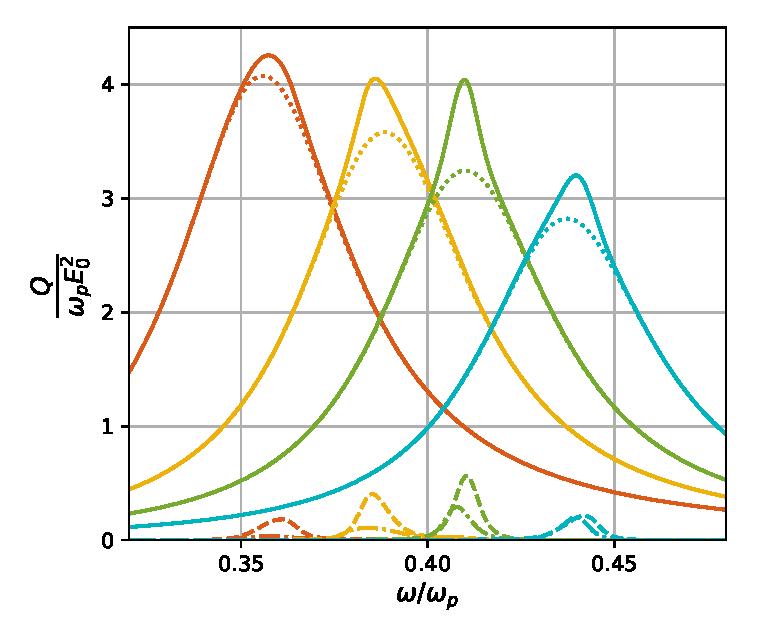
\includegraphics[width=80mm]{./image/fig1_epsd2.eps}
	\caption{Зависимость суммарной мощности потерь от частоты (сплошные кривые) для наночастицы с параметрами $v_F = 1.5 \cdot 10^8$ см/c, $\w_p = 5$ эВ, $\nu / \w_p = 0.02$,  $\eps_\infty= 2$ при различных значения диэлектрической проницаемости внешней среды. Кривым с резонансными пиками, расположенными слева-направо, отвечают значения $\eps_d = 4, 3, 2.5, 2$. Вклады от дипольной, монопольной и квадрупольной составляющих колебаний изображены точечными, пунктирными и штрих-пунктирными кривыми, соответственно.}
	\label{fig1_epsd2}
\end{figure} 
\newpage
\begin{figure}[h]
	\centering
	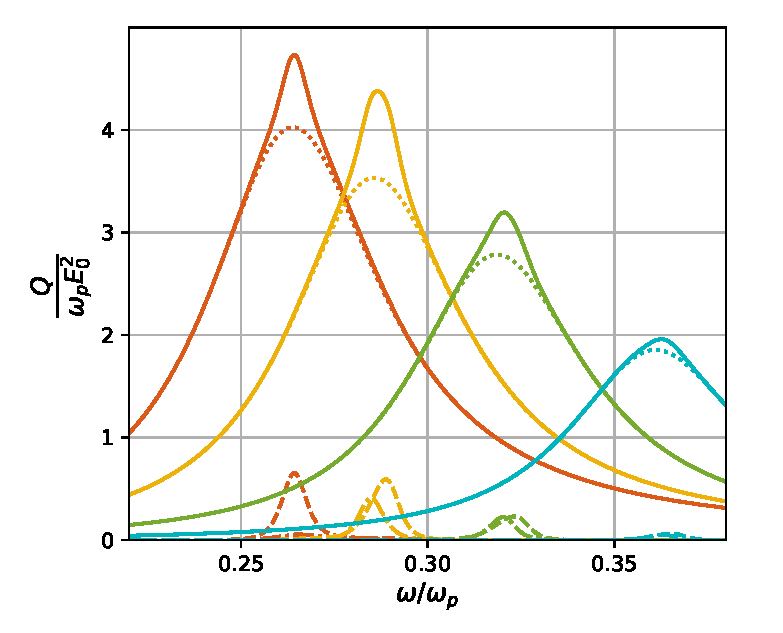
\includegraphics[width=80mm]{./image/fig1_epsd4.eps}
	\caption{ То же, что и на рисунке \ref{fig1_epsd2}, при $\eps_\infty= 4$.}
	\label{fig1_epsd4}
\end{figure} 
\newpage
\begin{figure}[h]
	\centering
	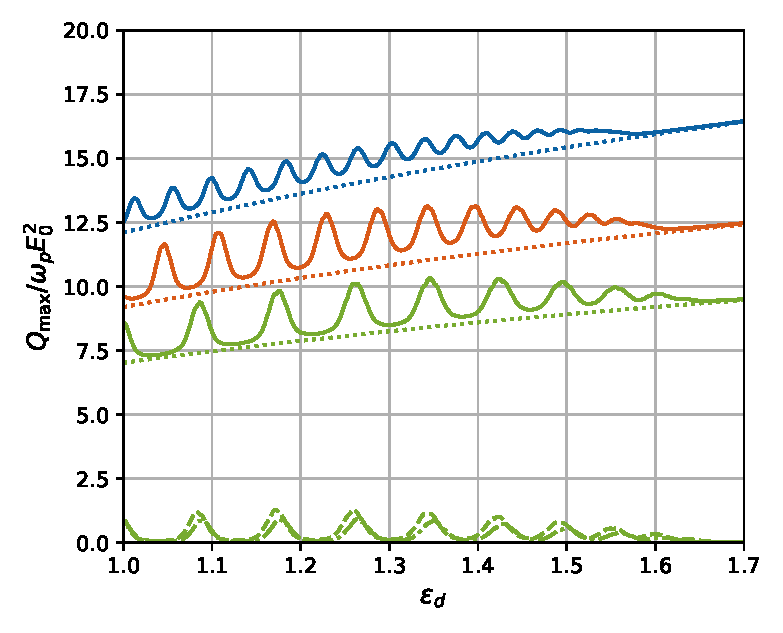
\includegraphics[width=80mm]{./image/natr2.eps}
	\caption{Зависимости максимальной мощности потерь для сферических наночастиц натрия (при $v_F = 1.07\cdot10^8$ см/с, $\w_p = 5.71$ эВ, $\nu = 0.03$ эВ \cite{ Blaber2009}) радиусом 10 нм и 7 нм при интенсивности внешнего поля $10^8$ $\text{Вт}/\text{см}^2$, и радиусом 5 нм при интенсивности $5 \cdot 10^7$ $\text{Вт}/\text{см}^2$ сверху вниз соответственно. Сплошной линией указана полная мощность потерь, точечной линией – вклад в потери от дипольных колебаний. В нижней части графика для наночастицы радиусом 5 нм пунктиром и штрих-пунктиром показан вклад от монопольных и квадрупольных колебаний соответственно.}

	\label{natr}
\end{figure} 
\end{document}
